\subsection{Simplicity of the alternating group ($A_n$)}
The following results are headed towards the proof of the simplicity of $A_n$ for $n \geq 5$. The 
way we will prove the simplicity of $A_n$ is by showing that every even permutation in $A_n$ can 
be expressed as a product of length-3-cycles for $n \geq 4$. Also, we will prove that every 
even permutation in $A_n$ can be expressed as a single length-3-cycle for $n \geq 5$. We will then 
say that every normal subgroup of $S_n$ that contains a length-3-cycle must contain all
length-3-cycles, hence every non-trivial normal subgroup of $A_n$ will contain at least 
one length-3-cycle, hence it will contain all of them, and so with their products, thus it 
will contain all even permutations, hence it will be equal to $A_n$. \\  

\begin{definition}[Simple group]
    A group $G$ is called simple if it has no non-trivial normal subgroups. In other words, the only 
    normal subgroups of $G$ are itself and $\{\epsilon\}$.
\end{definition} \vspace{0.2em}

\begin{theorem}
    If that $A_n$ is simple, There is no other non-trivial normal subgroup of $S_n$
\end{theorem}
\begin{proof}
    Let $H$ be a normal subgroup of $S_n$. Then, by lemma \ref{lem:intersectionOfNormalIsNormal}, we 
    have that $H \cap A_n$ is a normal subgroup of $A_n$ and since $A_n$ is simple, we have that 
    $H \cap A_n = \{\epsilon\}$ or $H \cap A_n = A_n$. \\

    If $H \cap A_n = \{\epsilon\}$, then $H$ is either the trivial subgroup or it is a group 
    with only odd permutations. Since $H$ must be a group, it must be closed under the 
    product of permutations, so it must contain the product of two odd permutations, which is an
    even permutation. Hence $H$ must contain an even permutation, which is a contradiction. \\

    If $H \cap A_n = A_n$, then $H$ contains $A_n$, so either they are identical or there 
    is an element of $S_n$ which is in $H$ but not in $A_n$. Suppose that $H$ is not
    identical to $A_n$. Then, the only element of $H$ that is not in $A_n$ must be an odd 
    permutation $\alpha$, but since $H$ is a group, it must be closed under the product of
    permutations, so it must contain $\alpha(A_n)$ which is to say that it has to contain 
    all products of even permutations with $\alpha$. \\  

    So we have that $H$ contains $\vv{f}(A_n)$ where $f$ is a function that takes an even
    permutation and returns itself multiplied by $\alpha$. The function is injective:

    $$ f(\sigma) = f(\tau) $$
    $$ \sigma \circ \alpha = \tau \circ \alpha  $$
    $$ \sigma \circ \alpha \circ \alpha^{-1} = \tau \circ \alpha \circ \alpha^{-1} $$
    $$ \sigma = \tau $$
    
    Also, since $f(\sigma)$ is an odd permutation, we can say that $\vv{f}(A_n)$ disjoint 
    from $A_n$. This means that $H$ contains two disjoint sets of permutations, both of which are
    of cardinality $|A_n|$ which implies that $|H| = 2|A_n| = |S_n|$ Hence $H$ is itself just $S_n$. \\

\end{proof} 
\vspace{0.4em}

\newpage

\begin{lemma}
    \label{lem:evenPermutationIsProductOfThreeCycles}
    Every even permutation in $A_n$ of length 2 can be expressed 
    as a product of length-3-cycles for $n \geq 4$.
\end{lemma}
\begin{proof}
    We can express every even permutation of length 2 in the form $(a,b) \circ (b,c)$ 
    as the product of two length-3-cycles $(a,b,c) \circ (1)$. So, without loss of generality,
    we can focus just on permutations of the form $(a,b) \circ (c,d)$.\\

    We can easily show that every permutation in the form $(a,b) \circ (b,c)$ can be 
    expressed as $(a, b, c)$, as shown below in figres \ref{fig:SwapTwo} and 
    \ref{fig:SwapTwoAs3Cycles} \\
\end{proof} \vspace{0.2em}

\begin{figure}[H]
\label{fig:SwapTwo}
    \centering
    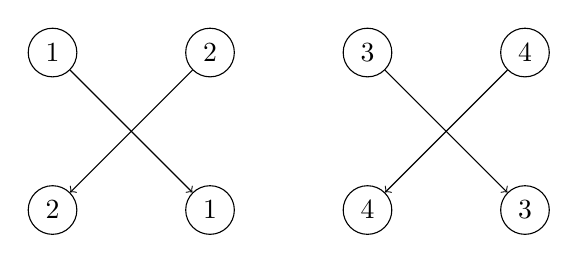
\begin{tikzpicture}
        
        \node (1-1) at (0, 0) [circle, draw] {1};
        \node (1-2) at (2, 0) [circle, draw] {2};
        \node (1-3) at (4, 0) [circle, draw] {3};
        \node (1-4) at (6, 0) [circle, draw] {4};
        
        \node (2-1) at (0, -2) [circle, draw] {2};
        \node (2-2) at (2, -2) [circle, draw] {1};
        \node (2-3) at (4, -2) [circle, draw] {4};
        \node (2-4) at (6, -2) [circle, draw] {3};

        \draw[->] (1-1) -- (2-2);
        \draw[->] (1-2) -- (2-1); 

        \draw[->] (1-3) -- (2-4);
        \draw[->] (1-4) -- (2-3); 

    \end{tikzpicture}
    \caption{The permutation $[(1,2) \circ (3,4)]$ }

\end{figure}

\begin{figure}[H]
\label{fig:SwapTwoAs3Cycles}
    \centering
    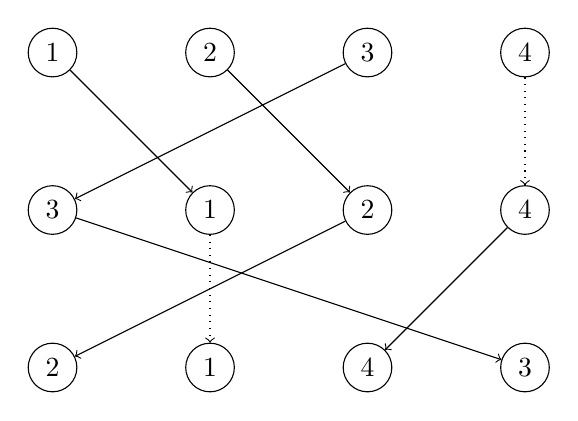
\begin{tikzpicture}
        
        \node (1-1) at (0, 0) [circle, draw] {1};
        \node (1-2) at (2, 0) [circle, draw] {2};
        \node (1-3) at (4, 0) [circle, draw] {3};
        \node (1-4) at (6, 0) [circle, draw] {4};
        
        \node (2-1) at (0, -2) [circle, draw] {3};
        \node (2-2) at (2, -2) [circle, draw] {1};
        \node (2-3) at (4, -2) [circle, draw] {2};
        \node (2-4) at (6, -2) [circle, draw] {4};

        \node (3-1) at (0, -4) [circle, draw] {2};
        \node (3-2) at (2, -4) [circle, draw] {1};
        \node (3-3) at (4, -4) [circle, draw] {4};
        \node (3-4) at (6, -4) [circle, draw] {3};

        \draw[->] (1-1) -- (2-2);
        \draw[->] (1-2) -- (2-3);
        \draw[->] (1-3) -- (2-1);
        \draw[dotted, ->] (1-4) -- (2-4);
        
        \draw[->] (2-1) -- (3-4);
        \draw[dotted, ->] (2-2) -- (3-2);
        \draw[->] (2-4) -- (3-3);
        \draw[->] (2-3) -- (3-1); 
 

    \end{tikzpicture}
    \caption{The permutation $[(1,2,3) \circ (1,4,3)]$ }

\end{figure} \vspace{0.4em}

\begin{lemma}
    Every even permutation in $A_n$ of arbitraty length can be expressed 
    as a product of length-3-cycles for $n \geq 4$.
\end{lemma}
\begin{proof}
    By definition, every even permutation of length $2k$ is a product of $2k$ length-2-cycles, which 
    are called prime-factors. We can consider them pairwise and define every even permutation 
    as a product of $k$ even permutations of length 2. Thanks to lemma 
    \ref{lem:evenPermutationIsProductOfThreeCycles} we can herby
    express every even permutation of length $2k$ as a product of $k$ length-3-cycles,
    thus proving the lemma. \\
\end{proof} \vspace{0.2em}

\newpage

\begin{lemma}
    \label{lem:everyThreeCycleIsInSubgroupsOfAN}
    Every normal subgroup $H \triangleleft S_n$ that contains a length-3-cycle must contain all 
    length-3-cycles given that $n \geq 3$.
\end{lemma}
\begin{proof}
    Assume $H \triangleleft S_n$ and that $H$ contains a length-3-cycle $(a,b,c)$. Then consider 
    that by definition of normality we have that the following statement holds true:

    $$ \forall \pi \in S_n\;\; \pi \circ (a,b,c) \circ \pi^{-1} \in H $$ \vspace{0.2em}

    We want to show that $H$ contains all length-3-cycles. So, for the arbitrary length-3-cycle
    $(i,j,k)$ we will show that we can find a permutation $\pi$ such that:

    $$ \pi \circ (a,b,c) \circ \pi^{-1} = (i,j,k) $$ \vspace{0.2em}

    In particular, such permutation $\pi$ exists and its defined by cases as shown below:

    \begin{equation*}
        h(x) = 
        \begin{cases*}
            a      & \text{if} \( x = i \)  \\
            b      & \text{if} \( x = j \)  \\
            c      & \text{if} \( x = k \)  \\
            x      & \text{otherwise}       \\
        \end{cases*}
    \end{equation*} \\
\end{proof}

\begin{lemma}
\label{lem:everyEvenPermutationIsInSubgroupsOfAN}
    Every normal subgroup $H \triangleleft S_n$ that contains an even permutation with exactly 2 
    prime factors must contain at least one length-3-cycle given that $n \geq 5$.
\end{lemma}
\begin{proof}
    Let $(a,b) \circ (c,d) \in H \triangleleft S_n$ be an even permutation. Since $H$ is normal:

    $$ \forall \pi \in S_n\;\; \pi \circ (a,b) \circ (c,d) \circ \pi^{-1} \in H $$ \vspace{0.2em}

    Sine $H$ is a group, it's closed under the product of its permutations, hence we can
    claim:

    $$ \forall \pi \in S_n\;\;\forall \sigma \in H\;\; \pi \circ \sigma \circ \pi^{-1} \circ \sigma^{-1} \in H $$
    $$ \forall \pi \in S_n\;\; \pi \circ (a,b) \circ (c,d) \circ \pi^{-1} \circ (d,c) \circ (b,a) \in H $$ \vspace{0.2em}

    If we take $\pi = (a,b) \circ (c, e)$ then we can express the whole thing as a length-3-cycle:

    \begin{align*} 
        \gamma \in H &= \pi \circ (a,b) \circ (c,d) \circ \pi^{-1} \circ (d,c) \circ (b,a)  \\
               &= (a,b) \circ (c, e) \circ (a,b) \circ (c,d) \circ (e, c) \circ (b,a) \circ (d,c) \circ (b,a) \\
               &= (e,c,d)
    \end{align*}
\end{proof}

A visualization of the above construction is shown in the following page in terms of 
permutation diagrams on $A_5$ where $a = 1$, $b = 2$, $c = 3$, $d = 4$, $e = 5$. \\

\newpage

\begin{figure}[H]
    \label{fig:SwapTwoAs3Cycles}
        \centering
        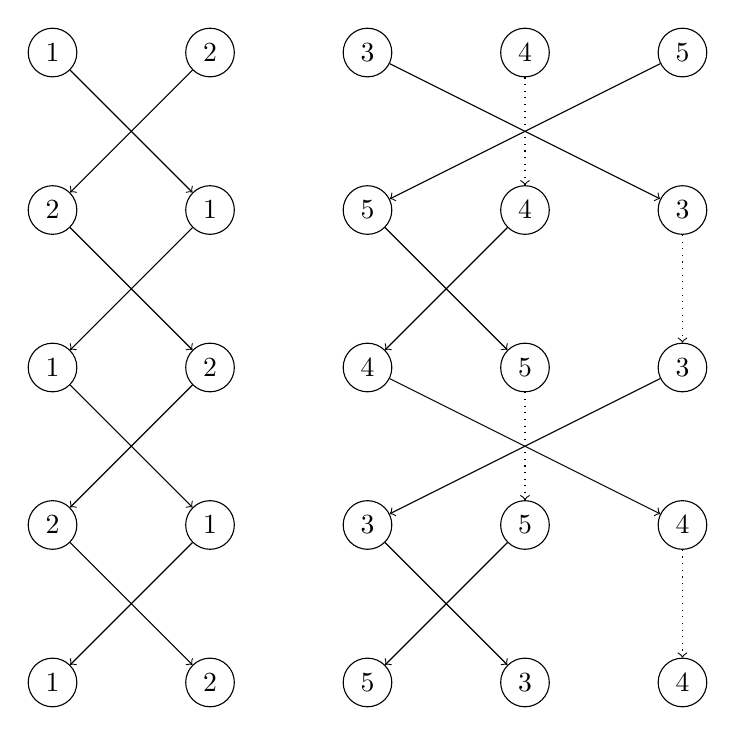
\begin{tikzpicture}
            
            \node (1-1) at (0, 0) [circle, draw] {1};
            \node (1-2) at (2, 0) [circle, draw] {2};
            \node (1-3) at (4, 0) [circle, draw] {3};
            \node (1-4) at (6, 0) [circle, draw] {4};
            \node (1-5) at (8, 0) [circle, draw] {5};
            
            \node (2-1) at (0, -2) [circle, draw] {2};
            \node (2-2) at (2, -2) [circle, draw] {1};
            \node (2-3) at (4, -2) [circle, draw] {5};
            \node (2-4) at (6, -2) [circle, draw] {4};
            \node (2-5) at (8, -2) [circle, draw] {3};

            \node (3-1) at (0, -4) [circle, draw] {1};
            \node (3-2) at (2, -4) [circle, draw] {2};
            \node (3-3) at (4, -4) [circle, draw] {4};
            \node (3-4) at (6, -4) [circle, draw] {5};
            \node (3-5) at (8, -4) [circle, draw] {3};

            \node (4-1) at (0, -6) [circle, draw] {2};
            \node (4-2) at (2, -6) [circle, draw] {1};
            \node (4-3) at (4, -6) [circle, draw] {3};
            \node (4-4) at (6, -6) [circle, draw] {5};
            \node (4-5) at (8, -6) [circle, draw] {4};

            \node (5-1) at (0, -8) [circle, draw] {1};
            \node (5-2) at (2, -8) [circle, draw] {2};
            \node (5-3) at (4, -8) [circle, draw] {5};
            \node (5-4) at (6, -8) [circle, draw] {3};
            \node (5-5) at (8, -8) [circle, draw] {4};
    
            \draw[->] (1-1) -- (2-2);
            \draw[->] (1-2) -- (2-1);

            \draw[->] (1-3) -- (2-5);
            \draw[->] (1-5) -- (2-3);
            
            \draw[dotted, ->] (1-4) -- (2-4);

            \draw[->] (2-1) -- (3-2);
            \draw[->] (2-2) -- (3-1);

            \draw[->] (2-3) -- (3-4);
            \draw[->] (2-4) -- (3-3);
            
            \draw[dotted, ->] (2-5) -- (3-5);

            \draw[->] (3-1) -- (4-2);
            \draw[->] (3-2) -- (4-1);

            \draw[->] (3-3) -- (4-5);
            \draw[->] (3-5) -- (4-3);
            
            \draw[dotted, ->] (3-4) -- (4-4);

            \draw[->] (4-1) -- (5-2);
            \draw[->] (4-2) -- (5-1);

            \draw[->] (4-3) -- (5-4);
            \draw[->] (4-4) -- (5-3);
            
            \draw[dotted, ->] (4-5) -- (5-5);
    
        \end{tikzpicture}
        \caption{Visualization of lemma \ref{lem:everyEvenPermutationIsInSubgroupsOfAN}}
    
    \end{figure} \vspace{0.4em}

Another way to refine the proof of lemma \ref{lem:everyEvenPermutationIsInSubgroupsOfAN} is to show 
that every $(a, b) \circ (x, y) = (x, y) \circ (a, b)$ as long as $x,y,a,b$ are all distinct. This 
means that we can refactor the equation as follows:

\begin{align*} 
    \pi\sigma\pi^{-1}\sigma^{-1} \in H 
        &= (a,b) \circ (c, e) \circ (a,b) \circ (c,d) \circ (e, c) \circ (b,a) \circ (d,c) \circ (b,a) \\
        &= (a,b) \circ (a,b) \circ (c, e) \circ (c,d) \circ (e, c) \circ (b,a) \circ (d,c) \circ (b,a) \\
        &= (a,b) \circ (a,b) \circ (b,a) \circ (b,a) \circ (c, e) \circ (c,d) \circ (e, c) \circ (d,c) \\
        &= \cancel{(a,b) \circ (a,b) \circ (b,a) \circ (b,a)} \circ (c, e) \circ (c,d) \circ (e, c) \circ (d,c) \\
        &= (c, e) \circ (c,d) \circ (e, c) \circ (d,c) \\
        &= (e,c,d)           
\end{align*}



\newpage
    

